\documentclass[tightpage, 26pt]{standalone}
\usepackage{tikz}

\begin{document}

 \begin{tikzpicture}\tikzstyle{every node}=[font=\huge]
    
   % Circles 
    \foreach \r in {1, 2,3,4}
      \draw[black, thick] (0,0) circle (\r) ;

   % Fill cirlces
    \draw[fill=green!40] (0,0) circle (1cm);
    \draw[fill=red!40] (0,0) circle (2cm) (0:1) arc (0:-360:1) ;
    \draw[fill=blue!40] (0,0) circle (3cm) (1:2) arc (1:-360:2) ;
    \draw[fill=yellow!40] (0,0) circle (4cm) (2:3) arc (2:-360:3) ;

    % Rays
    \foreach \a in {0, 180}
      \draw[thick,black] (\a:1) -- (\a:4);   

    \foreach \a in {90, 270}
      \draw[thick,black] (\a:1) -- (\a:2);

    \foreach \a in {60, 120, 240, 300}
      \draw[thick,black] (\a:2) -- (\a:4); 

    % Draw numbers
    \draw[black, thick] (0,0) node{$17$};

    \foreach \a in {13,14,15,16}
      \draw[black, thick] (-1125+ 90*\a:1.5) node{$\a$};
      % 45 + 90*(\a-13) = -1125 + 90*\a

    \foreach \a in {7,8,9,10,11,12}
      \draw[black, thick] (-390+ 60*\a:2.5) node{$\a$};
      % 30 + 60*(\a-7) = -390 + 60*\a

    \foreach \a in {1,2,3,4,5,6}
      \draw[black, thick] (-30+ 60*\a:3.5) node{$\a$};
      % 30 + 60*(\a-1) = -30 + 60*\a
  

    % Draw lines 
    \draw[<->,thick,blue, dashed] (210:5) -- (30:5);
    \draw[<->,thick,green, dashed] (270:5) -- (90:5);
    \draw[<->,thick,red, dashed] (150:5) -- (330:5);

    \draw[black, thick] (30:6) node{Anterior};
    \draw[black, thick] (90:5.5) node{AnteroSeptal};
    \draw[black, thick] (150:6) node{Septal};
    \draw[black, thick] (210:6) node{Inferior};
    \draw[black, thick] (270:5.5) node{Posterior};
    \draw[black, thick] (330:6) node{Lateral};


    \node[inner sep=0pt] (legend) at (6,0)
    {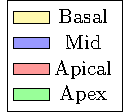
\includegraphics[width=.25\textwidth]{legend}};


    % Draw RV
    \draw [red,very thick,domain=60:180] plot ({4.3*cos(\x)}, {4.3*sin(\x)});
    \draw[red, thick] (-3.0,3.9) node{RV};

\end{tikzpicture}
\end{document}
%%% Local Variables:
%%% mode: latex
%%% TeX-master: t
%%% End:
